\documentclass{beamer}
\usetheme{CambridgeUS}
\usepackage[utf8]{inputenc}
\usepackage{graphicx}
\usepackage{tikz}

% Logo top-right
\logo{
\includegraphics[height=0.8cm]{HTL-logo.jpeg}} % Replace with correct path to HTL Anichstraße logo

% Title and author info
\title[AI Integration in Education and Dev]{Integration of Artificial Intelligence in Education and Software Development}
\author[Luna Sch\"atzle, Florian Prandstetter]{Luna Sch\"atzle \\ Florian Prandstetter}
\institute[HTL Anichstra\ss e]{HTL Anichstra\ss e, Department of Business Informatics\\Thesis Supervisor:\\Mag. Dr. Dipl. -Ing. Albert Greinöcker\\MMag.a Eva-Maria Egger, MA}
\date{Diploma Thesis Defense -- April 2025}

\begin{document}

\begin{frame}
  \titlepage
\end{frame}

% Slide: Introduction
\begin{frame}{Introduction}
    \begin{itemize}
      \item \textbf{Presenter:} Luna Schätzle – Project Lead (AI evaluation, backend \& website)
      \item \textbf{Objective:} Open-source AI platform for education
      \item \textbf{Focus:} Evaluate various AI models for multiple use cases
      \item \textbf{Platform:} Enable students to access and experiment with AI
      \item \textbf{Motivation:} Overcome high resource requirements of current Open Source AI models
    \end{itemize}
  \end{frame}
  

% Slide: Project Team and Organization
\begin{frame}{Project Team and Management}
    \begin{itemize}
      \item \textbf{Team Members:} Luna Schätzle, Florian Prandstetter
      \item \textbf{Project Coordination:} Regular meetings, discussions, and planning sessions
      \item \textbf{Tools Employed:}
        \begin{itemize}
          \item GitHub for version control and collaborative coding
          \item Discord for communication and coordination
          \item Google Sheets for time tracking
          \item LaTeX for comprehensive documentation
        \end{itemize}
    \end{itemize}
  \end{frame}
  
% Slide: Theoretical Background
\begin{frame}{Theoretical Background}
    \begin{itemize}
      \item \textbf{LLMs Integration:} Evaluation and incorporation of various Large Language Models.
      \item \textbf{Interfaces:} API connections, local models (e.g., Ollama), and OpenAI API.
      \item \textbf{Evaluation:} Systematic testing of open source models 
    \end{itemize}
  \end{frame}
  

% Slide: Testing and Evaluation
\begin{frame}{Testing and Evaluation}
  \begin{itemize}
    \item Evaluation of models: Llama3.2, Deepseek-r1, gemma2, qwen, ...
    \item Testing methods: Different prompts and tasks where asked the models (automated via Python script)
    \item Evaluation criteria: 
      \begin{itemize}
        \item response time
        \item accuracy
        \item resource usage
        \item BLEU score
        \item readability
        \item Textquality
      \end{itemize}
  \end{itemize}
\end{frame}

%Maby extra slide with the results
\begin{frame}{Evaluation Results: Quantitative metrics}
  \begin{figure}
    \centering
    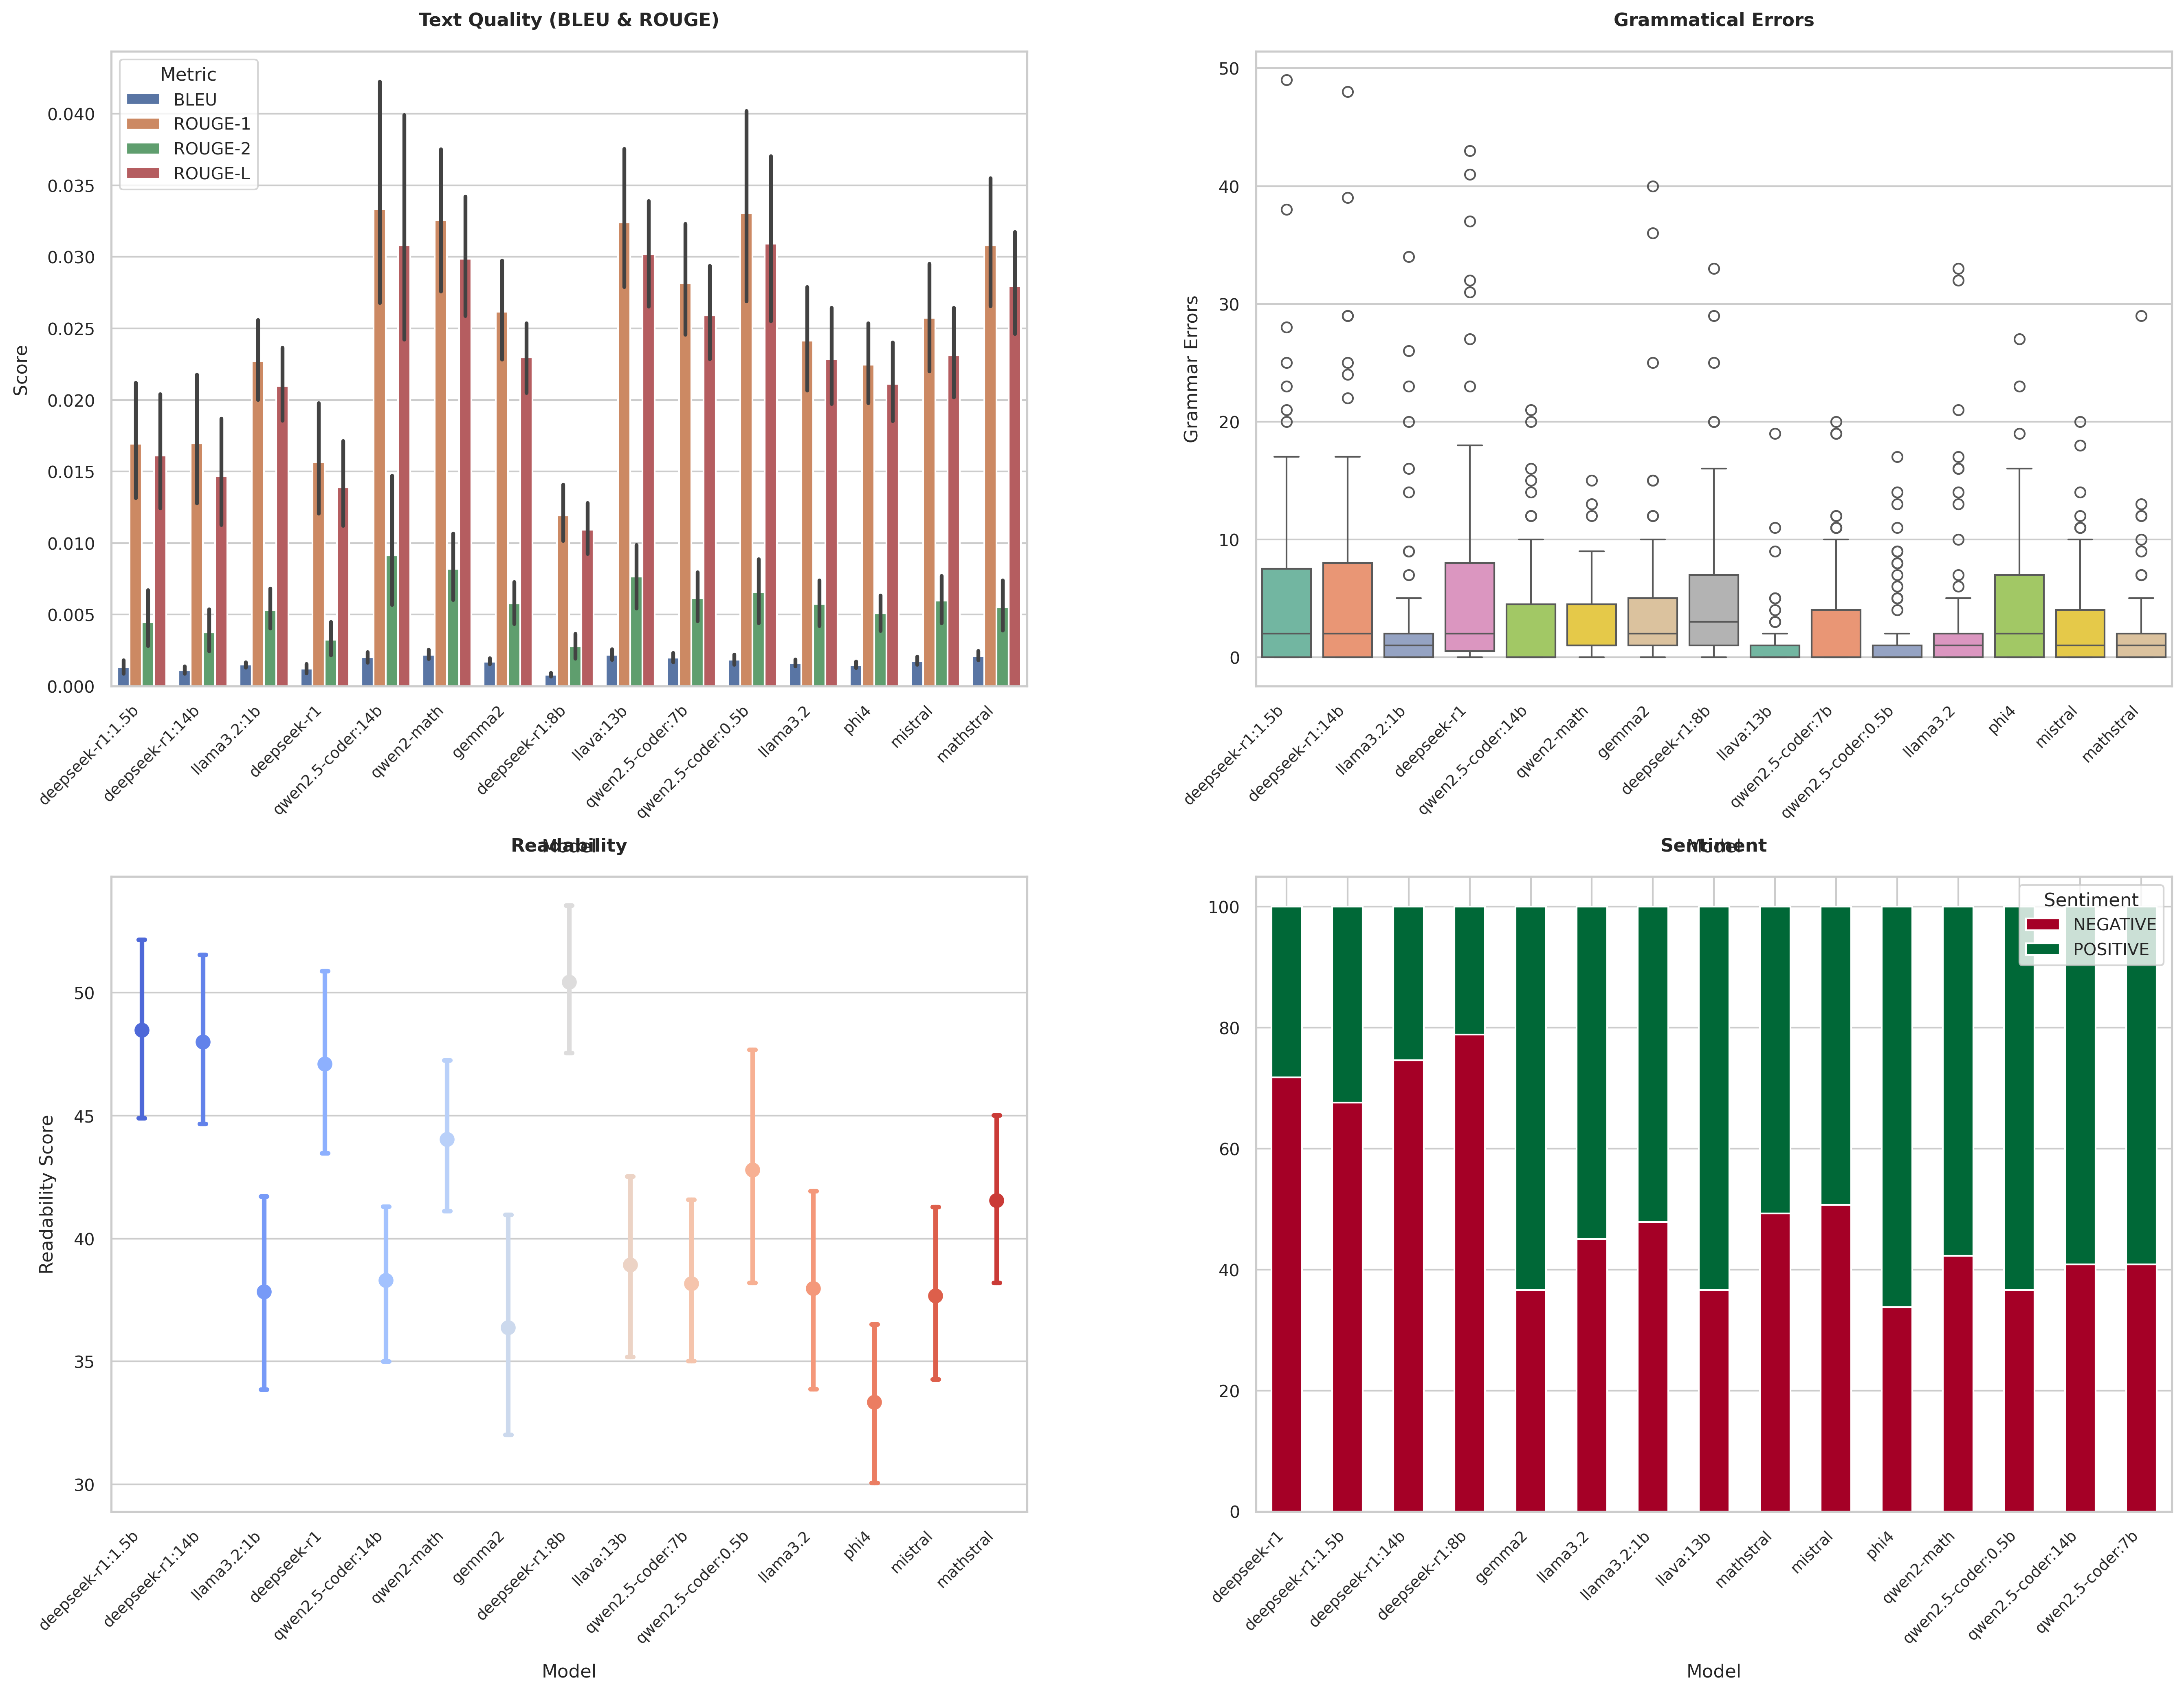
\includegraphics[width=0.8\textwidth]{combined_metrics.png}
    \caption{Evaluation Results of AI Models}
    \label{fig:evaluation-results}
  \end{figure}
\end{frame}

\begin{frame}{Evaluation Results: Qualitative metrics}
  \begin{columns}[t]
    \column{0.5\textwidth}
      \begin{figure}
        \centering
        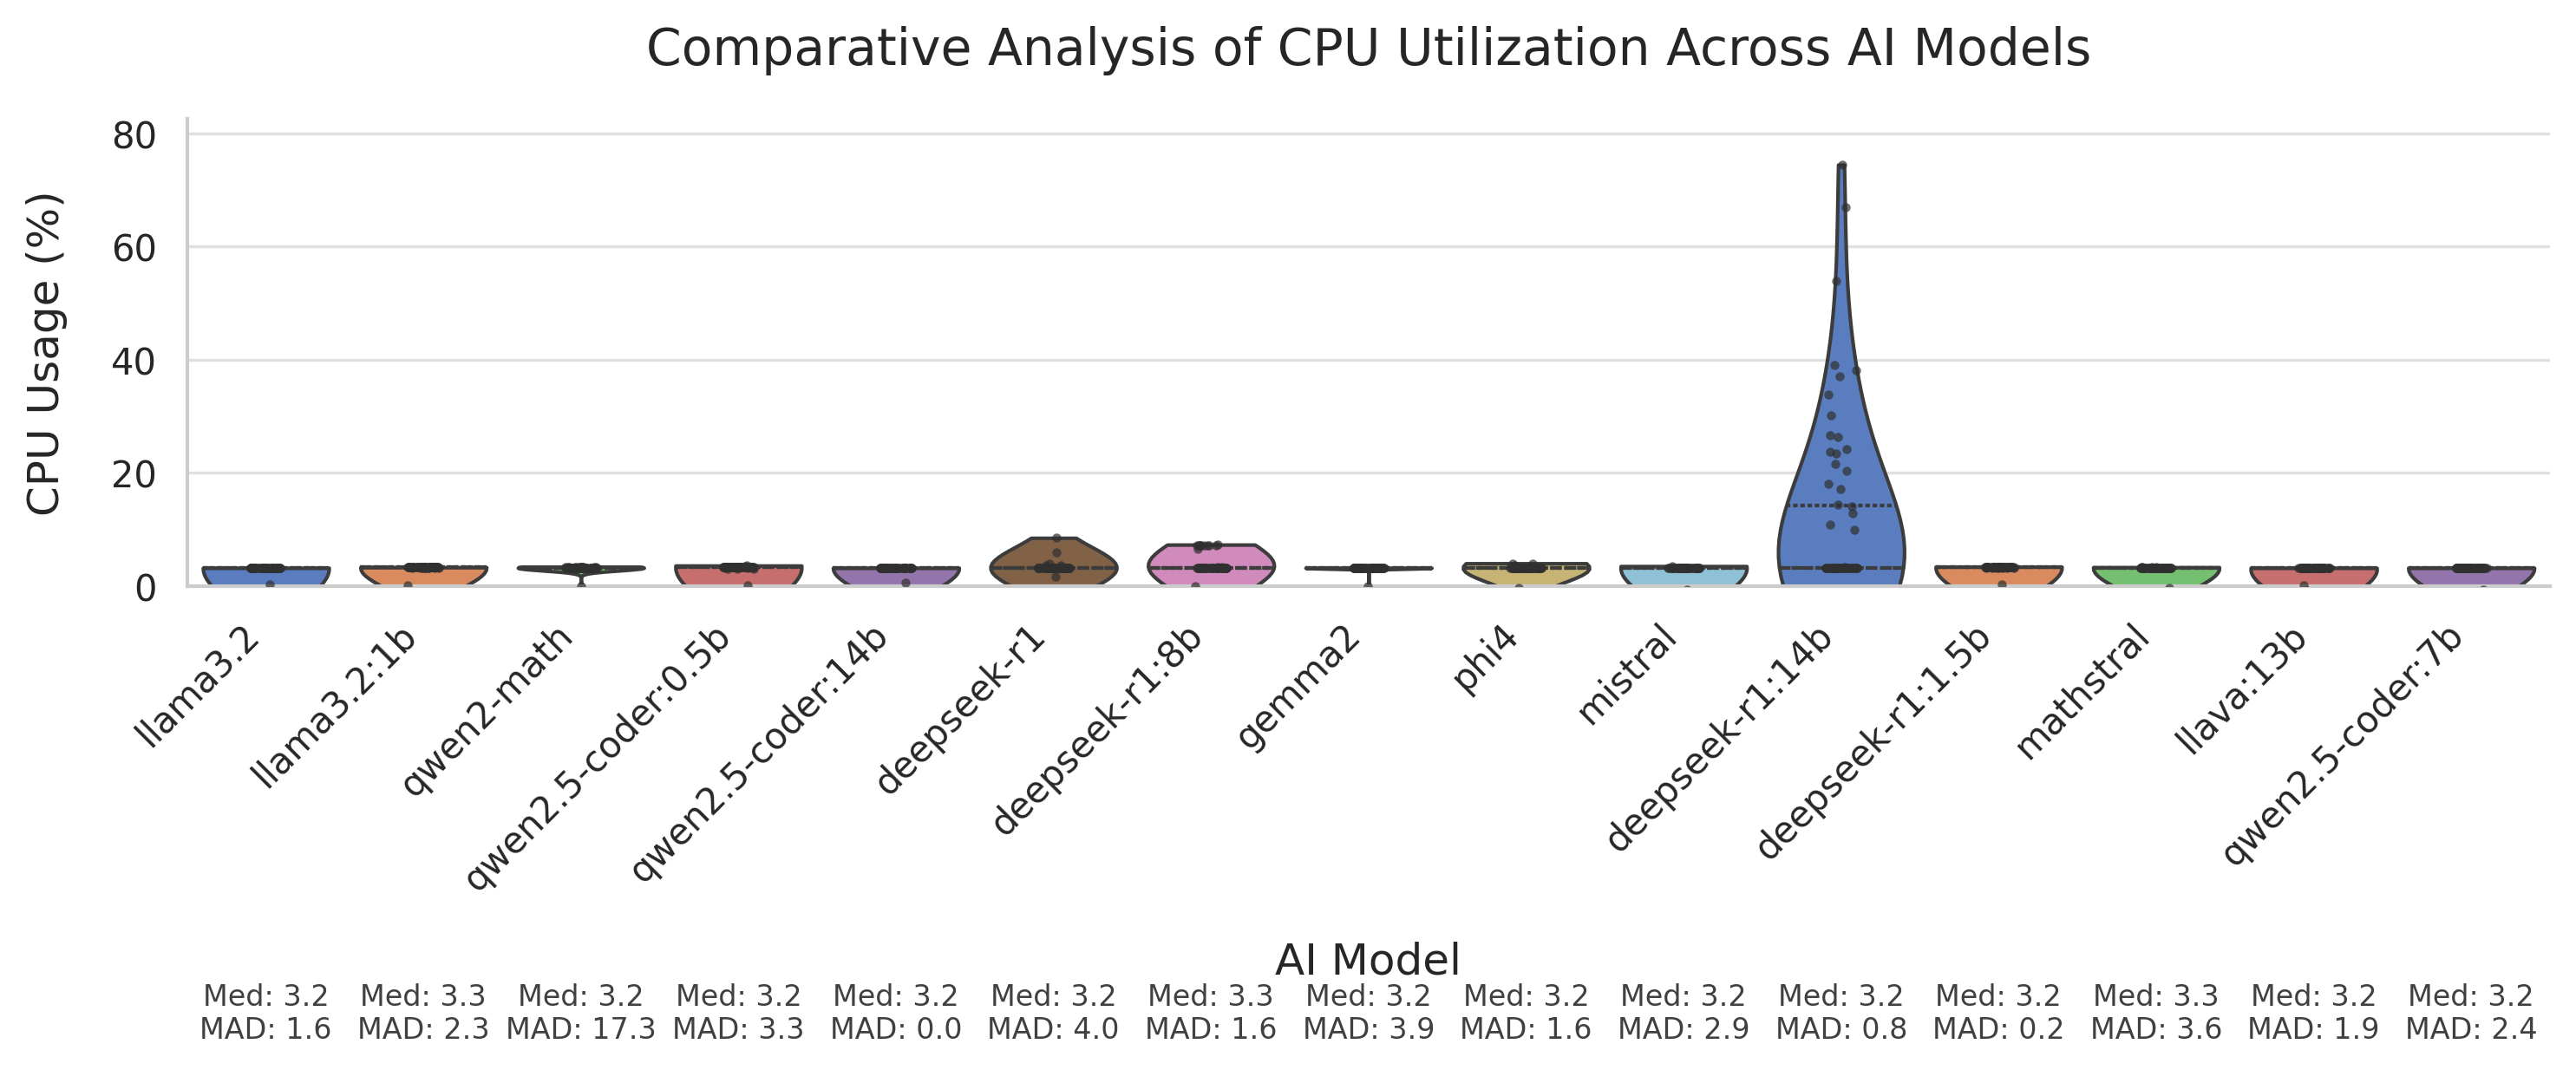
\includegraphics[width=0.9\columnwidth]{model_cpu_usage_comparison.png}
        \caption{CPU Usage Comparison}
        \label{fig:cpu-usage}
      \end{figure}
    \column{0.5\textwidth}
      \begin{figure}
        \centering
        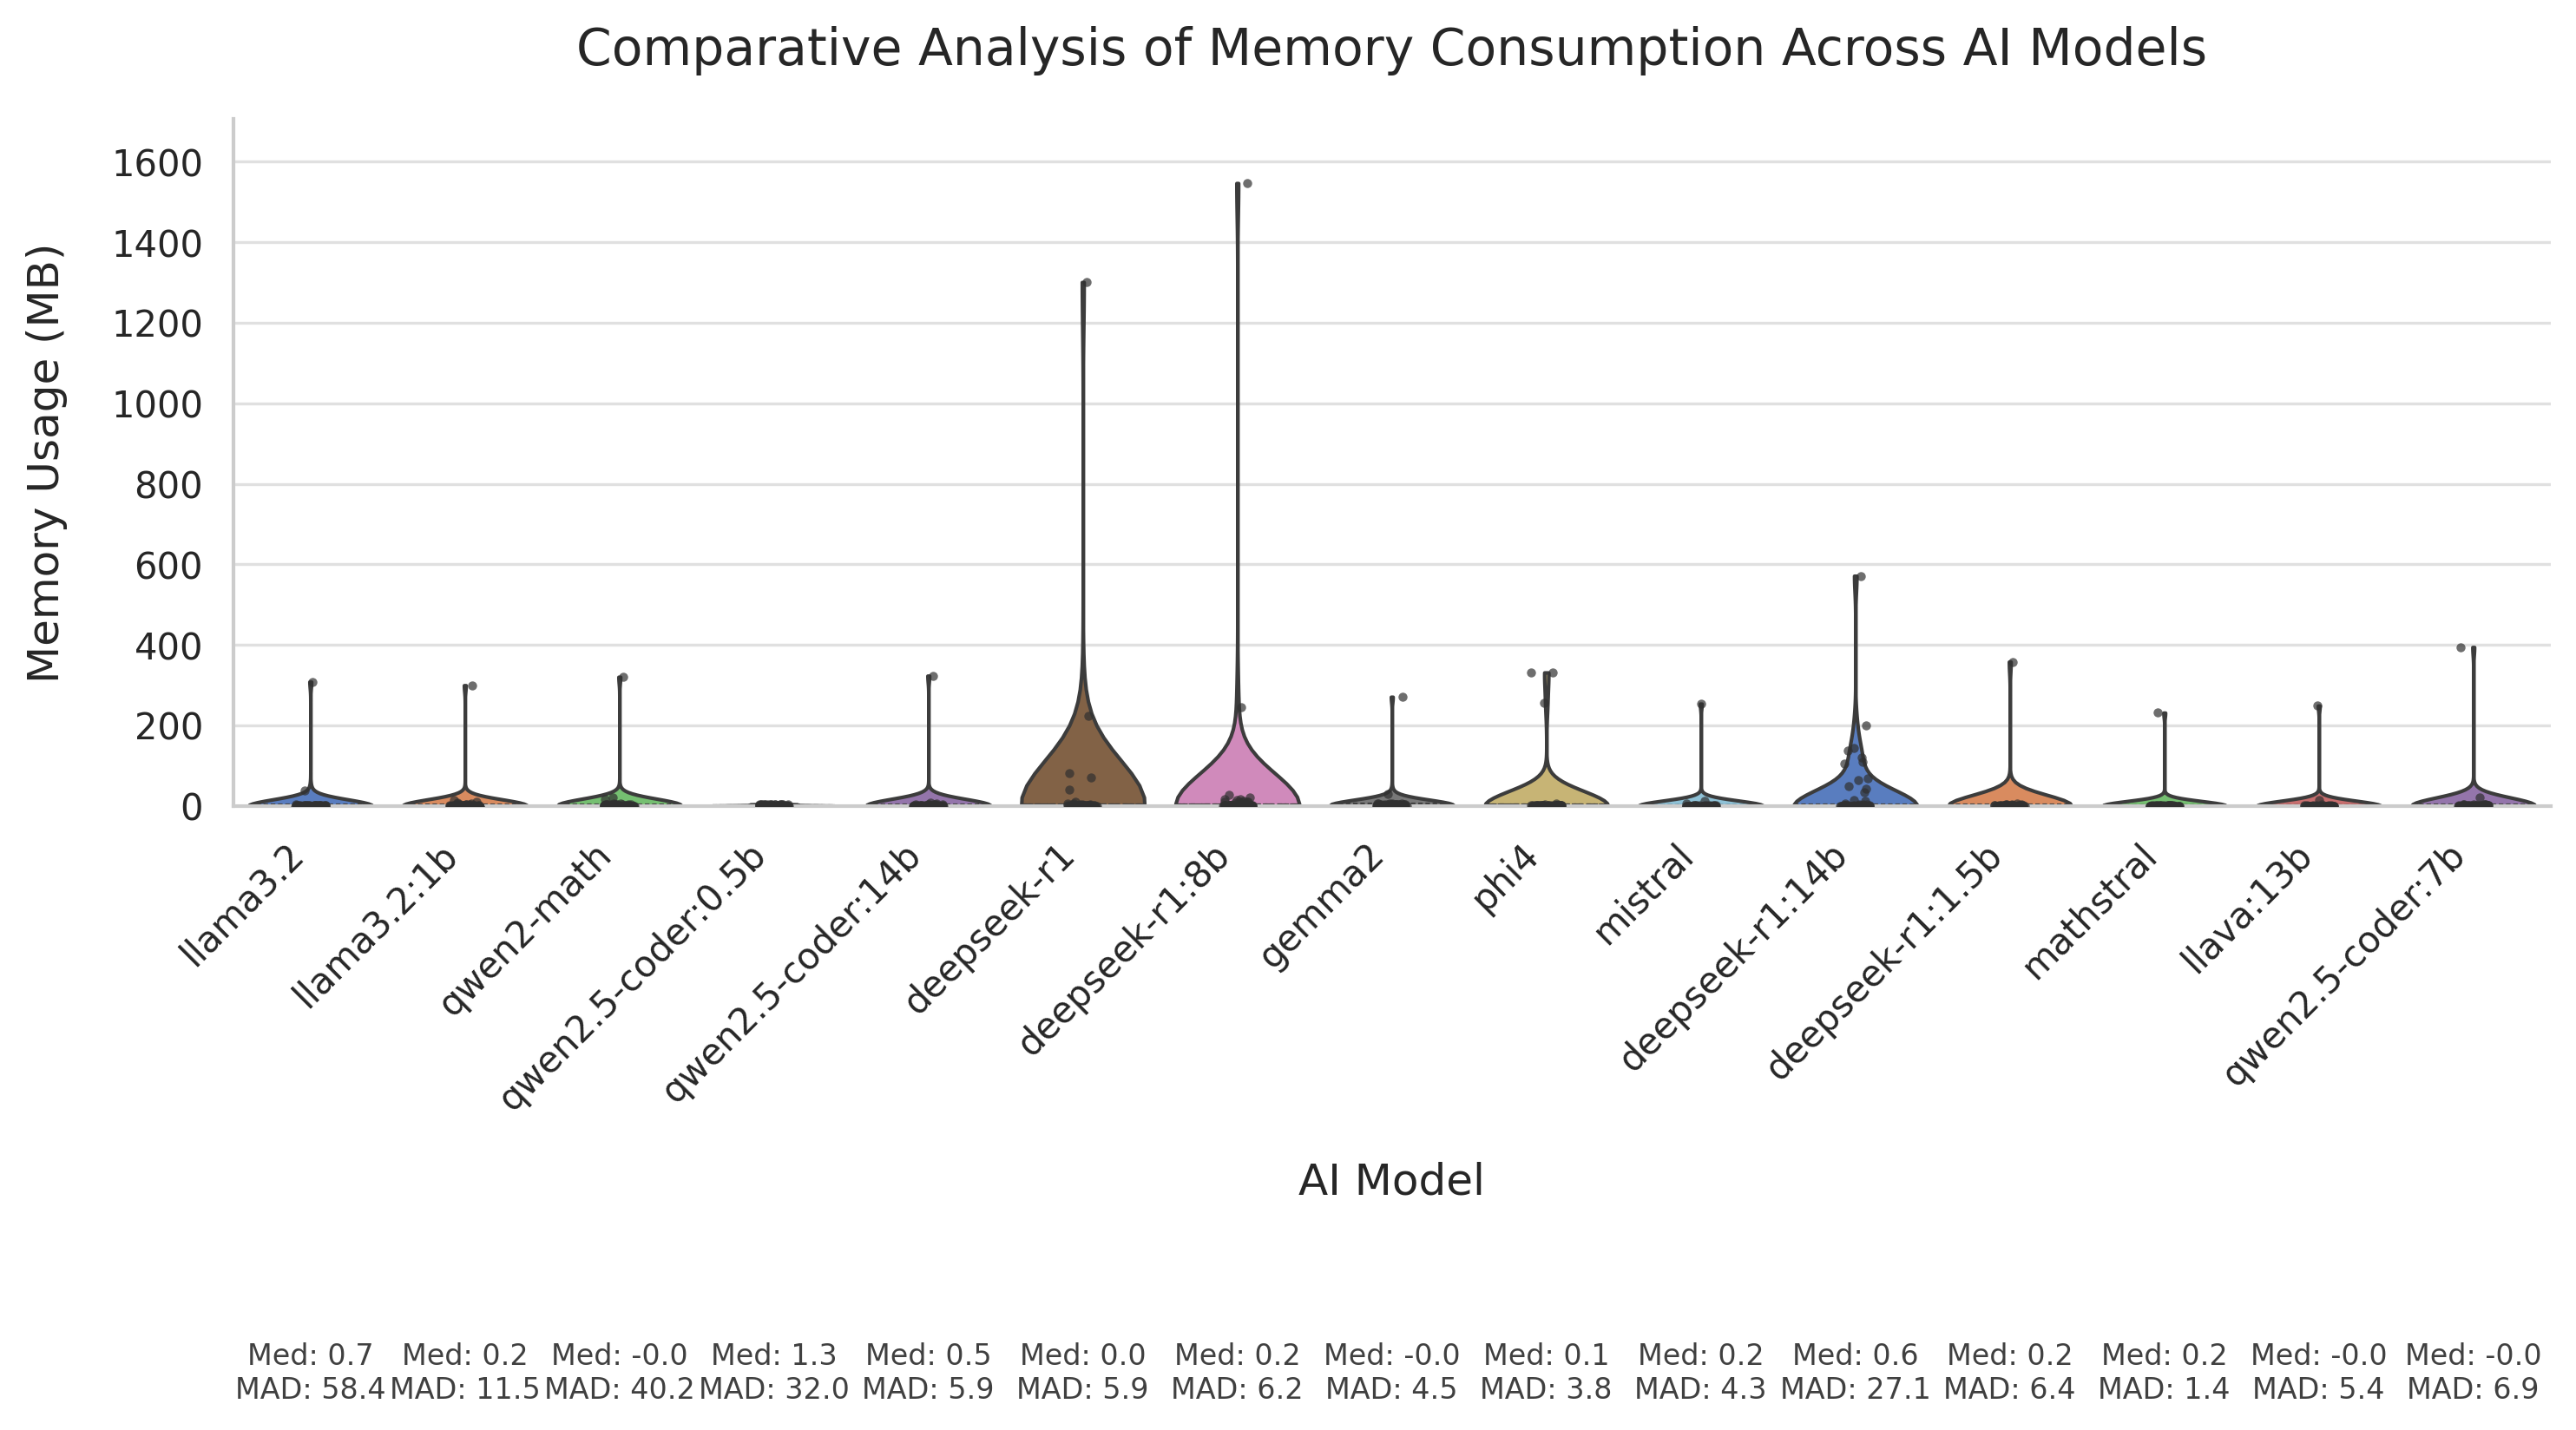
\includegraphics[width=0.9\columnwidth]{model_memory_usage_comparison.png}
        \caption{Memory Usage Comparison}
        \label{fig:memory-usage}
      \end{figure}
  \end{columns}
\end{frame}

% Slide: Backend Architecture
%\begin{frame}{Backend Architecture}
%  \begin{itemize}
%    \item Design based on model integration needs
%    \item Functionality of the backend (AI Hub, Code Bot)
%    \item Structure: Flask-based API, endpoints for services
%    \item Reference to server setup by Florian
%  \end{itemize}
%\end{frame}

% Slide: Website and Frontend
\begin{frame}{Website Platform}
  \begin{itemize}
    \item To realise the vision of the project, we created a website platform. 
    \item The website was realised thru the use of Vue.js and Flask (Backend API) and Firebase (Database).
    \item The website has the following features (as of the presentation date):
    \begin{itemize}
      \item User registration, login and profile management
      \item Chatbot interface a various AI models (thrue API general local models, Programming Assistant, Chat with chat GPT, image regocnition via LLaVA and Llama3.2-vision)
      \item Image generation with DallE
      \item OCR (Optical Character Recognition) with Tesseract and enhanced via LLama3.2
    \end{itemize}
    \end{itemize}
\end{frame}

% Slide: AI in Economics and Ethics
\begin{frame}{AI in Economics and Ethics}
\textbf{Applications:}
        \begin{itemize}
          \item Customer service \& support
          \item Supply chain management
          \item Predictive analytics
          \item Data analysis
          \item Process automation
        \end{itemize}

\end{frame}

% Slide: AI in Economics and Ethics
\begin{frame}{AI in Economics and Ethics}
\textbf{Ethical \& Social Concerns:}
        \begin{itemize}
          \item Bias in training data
          \item Transparency \& accountability
          \item Privacy and data protection
          \item Impact on employment
        \end{itemize}
\end{frame}

% Slide: AI in Economics and Ethics
\begin{frame}{AI in Economics and Ethics}
\textbf{Regulatory Challenges:}
            \begin{itemize}
                \item Inconsistent global regulations 
                \item EU AI Act considerations [EUR-Lex: 2024/1689]
                \item Data security standards (e.g., GDPR [EUR-Lex: 2016/679])
            \end{itemize}
\end{frame}




% Slide: Open Source in an Economic Context
% Slide 1: Open Source Overview
\begin{frame}{Open Source Overview}
    \begin{itemize}
      \item \textbf{Definition:} Collaborative, transparent development with public source code.
      \item \textbf{Advantages:} Cost efficiency, flexibility, improved security through peer review, high compatibility.
      \item \textbf{Economic Impact:} \\
        \quad -- Drives innovation \& cross-industry collaboration \\
        \quad -- Empowers startups and lowers entry barriers
    \end{itemize}
  \end{frame}
  
  % Slide 2: Challenges & Application
  \begin{frame}{Challenges and Revenue Models}
    \begin{itemize}
      \item \textbf{Challenges:} Fragmentation, limited support, licensing complexities, security risks.
      \item \textbf{Revenue Models:} Open core, managed services, support contracts, donations, dual licensing.
      \item \textbf{Our Approach:} Utilize open source tools (e.g., Python, Flask, Vue.js) under GNU GPL-3.0 for transparency and collaboration.
    \end{itemize}
  \end{frame}
  


% Slide: Conclusion
\begin{frame}{Conclusion}
  \begin{itemize}
    \item Summary of achievements
    \item Insights gained during the development
    \item Future potential of the system
    \item Final thoughts and acknowledgments
  \end{itemize}
\end{frame}

\begin{frame}{Florian}
  
\end{frame}

\end{document}
